% TIMM: Temporal Influence Maximization via Reverse Reachable Sampling
%       under Hawkes Processes
% ICDM 2026 Submission

\documentclass[10pt,conference]{IEEEtran}
\pagestyle{empty}
\usepackage{graphicx,amsmath,amssymb,amsthm,algorithm,algpseudocode}
\usepackage{booktabs,multirow,hyperref,color,xspace}
\hypersetup{hidelinks}
\usepackage[mathscr]{euscript}

\newtheorem{theorem}{Theorem}
\newtheorem{lemma}{Lemma}
\newtheorem{corollary}{Corollary}
\newtheorem{conjecture}{Conjecture}
\newtheorem{definition}{Definition}
\newcommand{\tiimm}{TIMM\xspace}
\newcommand{\trr}{TRR\xspace}
\newcommand{\esr}{ESR\xspace}

\begin{document}

\title{TIMM: Temporal Influence Maximization via Reverse Reachable Sampling\\ under Hawkes Processes}

\author{\IEEEauthorblockN{Anonymous}}

\maketitle

\begin{abstract}
Influence maximization on temporal networks requires modeling when events occur, not only which edges exist.
We study continuous-time influence maximization under exponential Hawkes diffusion and propose \tiimm{}, a reverse-sampling algorithm based on \emph{Temporal Reverse Reachable (TRR) sets}.
TRR-set activation probabilities are derived from the Hawkes conditional intensity integral, enabling scalable reverse sampling for temporal cascades.
We prove strict monotonicity of temporal influence and establish a martingale concentration bound for TRR-set coverage estimates, while separating these rigorous results from the unresolved question of full submodularity under coupled Hawkes dynamics.
To assess the submodularity gap empirically, we introduce a sampled diagnostic based on random $(S,T,x)$ triples and calibrate TRR estimates against forward Monte Carlo simulation.
Across four real-world temporal networks spanning social media, citation, and online discussion domains, \tiimm{} consistently matches or outperforms static and snapshot baselines, with the largest gains on datasets exhibiting strong temporal burstiness.
On small graphs where a direct Monte Carlo Hawkes baseline is computationally feasible, \tiimm{} achieves comparable seed quality at a fraction of the runtime.
These results suggest that continuous-time reverse sampling is a practical route to scalable temporal influence maximization under specified Hawkes parameters.
\end{abstract}

%========================================================================
\section{Introduction}
%========================================================================

Information cascades in social media unfold in \emph{continuous time}.
A tweet goes viral within minutes, decays over hours, and may reignite when reshared by an influencer.
These temporal dynamics — burst, decay, and self-excitation — are not edge cases but the defining structure of real-world propagation.
Yet the theoretical foundations of Influence Maximization (IM) rest almost entirely on \emph{static} diffusion models where edge probabilities are constants, time is absent, and the rich sequential structure of cascades is discarded.

The cost of ignoring time is empirically significant: temporal-network IM studies show that the timing and ordering of interactions can materially change seed quality and diffusion outcomes~\cite{yanchenko2024}.
However, continuous-time temporal IM currently occupies a theoretical no-man's-land:
discrete snapshot methods~\cite{ohsaka2016} offer per-window guarantees but miss intra-window burst dynamics;
Monte Carlo greedy under Hawkes diffusion captures continuous-time decay but lacks an approximation guarantee and scales poorly beyond small graphs.

\textbf{The core challenge.}
Extending the RIS framework to continuous time requires simultaneously solving three problems:
(1)~defining a temporal reverse-sampling primitive whose activation probabilities faithfully mirror the forward Hawkes cascade;
(2)~proving singleton unbiasedness of this primitive under $\mu{=}0$ and validating multi-seed coverage empirically; and
(3)~establishing a concentration bound on the required number of temporal samples.
The submodularity of the temporal influence function — the property that enables the $(1-1/e-\varepsilon)$ approximation — is a further, deeper theoretical question.

\textbf{Our contributions.}
This paper makes progress on all fronts:

\begin{enumerate}
\item \textbf{TRR-set sampling primitive (\S5.1).}
We define the Temporal Reverse Reachable (TRR) set, a novel sampling primitive that extends RIS to continuous time.
The key insight is that the backward edge activation probability
$p = 1 - \exp(-\frac{\alpha}{\beta}(1 - e^{-\beta(\tau-t)}))$ 
is derived directly from the Hawkes conditional intensity integral, not heuristically assigned.
We prove that TRR-sets provide an unbiased estimator of \emph{singleton} temporal influence (Lemma~2) under the exponential Hawkes kernel with zero exogenous intensity ($\mu=0$), and establish a martingale concentration bound on the required number of TRR-sets (Theorem~1).

\item \textbf{Martingale-based sampling bound (\S5.2).}
Adapting the IMM martingale framework~\cite{tang2015} to temporal reverse walks, we prove that
$\theta = O(n \log(1/\delta) / \varepsilon^2)$ TRR-sets suffice for $(\varepsilon,\delta)$-concentration of the TRR coverage objective (Theorem~1).
This bound depends only on the unbiasedness of TRR-sets (Lemma~2) and standard concentration — it is \emph{independent} of submodularity.

\item \textbf{Submodularity analysis with empirical safeguards (\S4).}
We prove \textbf{strict monotonicity} of temporal influence under the exponential Hawkes kernel (Lemma~1).
We analyze the submodularity question through Ogata's thinning construction, identify the known technical gap in the coupling argument, and provide:
(a)~a theoretical analysis of containment under ``cascade tree monotonicity,''
(b)~statistical validation via the TRR-set estimator (0 violations in 500+ trials per dataset; upper 95\% CI on violation rate $<$0.74\%),
and (c)~the \emph{Empirical Submodularity Ratio} (ESR) — a per-dataset diagnostic that assesses the observed degradation from exact submodularity on sampled triples.
We frame submodularity as \textbf{Conjecture~1} and explicitly state which results depend on it.

\item \textbf{Comprehensive experimental validation (\S6).}
On real-world temporal networks spanning three orders of magnitude in size (1.9K--256K nodes, up to 355K temporal edges) across three domains (social media, citation, online discussion),
\tiimm{} achieves 8--50\% gains over StaticIMM on datasets where temporal dynamics matter, remains competitive in dense saturation regimes, runs 263$\times$ faster than our MC-Hawkes-Greedy baseline, and reveals systematic weaknesses of discrete snapshot methods on both bursty and non-bursty temporal data.
\end{enumerate}

\textbf{Paper positioning.}
Claims supported by proof (unbiasedness, martingale bound) are distinguished from those contingent on Conjecture~1 (full submodularity) or supported empirically (ESR).
The TRR-set primitive and the \tiimm{} algorithm provide a scalable reverse-sampling framework with singleton unbiasedness ($\mu{=}0$) and empirically calibrated multi-seed coverage, applicable to continuous-time temporal IM regardless of the submodularity conjecture's ultimate resolution.

%========================================================================
\section{Related Work}
%========================================================================

We briefly position our work against the most relevant IM literature.

\textbf{Static IM with guarantees.}
Kempe et al.~\cite{kempe2003} established the $(1-1/e)$ greedy approximation under submodular influence functions.
The RIS revolution — Borgs et al.~\cite{borgs2014}, Tang et al.~\cite{tang2014,tang2015}, Nguyen et al.~\cite{nguyen2016} — replaced forward Monte Carlo with reverse sampling, achieving near-linear time with $(1-1/e-\varepsilon)$ guarantees on billion-edge graphs.
\textit{Limitation:} All assume static graphs; temporal information is aggregated away or discarded.

\textbf{Temporal and dynamic IM.}
Ohsaka et al.~\cite{ohsaka2016} partition time into discrete windows, offering per-window guarantees but missing intra-window dynamics.
Continuous-time diffusion models have been studied for influence maximization and scalable influence estimation~\cite{gomez2012,du2013}.
These models highlight the importance of temporal transmission dynamics, but they do not provide a scalable reverse-sampling algorithm for coupled Hawkes self-exciting cascades.
Temporal-network IM has also been surveyed as a distinct problem class in which temporal ordering, observation windows, and seed timing alter both objective value and algorithm design~\cite{yanchenko2024}.
Saha et al.~\cite{saha2025} study hyperparametric robust dynamic IM but operate in discrete time with sliding windows.

\textbf{Our position.}
\tiimm{} is, to our knowledge, among the first algorithms to combine \emph{continuous-time} temporal modeling (Hawkes process) with \emph{rigorous sampling bounds} (martingale concentration) and \emph{empirical submodularity diagnostics} (ESR-based evidence).
Table~\ref{tab:positioning} summarizes the landscape.

\begin{table}[t]
\centering
\caption{Positioning in temporal IM literature.}
\label{tab:positioning}
\footnotesize
\setlength{\tabcolsep}{4pt}
\begin{tabular}{@{}lccr@{}}
\toprule
Method & Diffusion & Bound type & Max $n$ \\
\midrule
Ohsaka et al.~\cite{ohsaka2016} & Snap-IC & Window$^\dagger$ (1--1/$e$) & $10^5$ \\
CT-IM~\cite{gomez2012,du2013} & CT-IC & MC/est. & $10^6$ \\
MC-Hawkes (ours) & Hawkes (exp) & None & $\sim$500$^\ddagger$ \\
\textbf{\tiimm{} (this work)} & \textbf{Hawkes (exp)} & \textbf{ESR}$^*$ (empirical) & $\mathbf{2.6\times10^5}$ \\
\bottomrule
\end{tabular}\\[3pt]
$^\dagger$Per snapshot window. \; $^\ddagger$Our re-implementation. \; $^*$ESR: sampled diagnostic; 0 violations in 500+ trials (upper 95\% CI on violation rate $<$0.74\%).
\end{table}

%========================================================================
\section{Preliminaries}
%========================================================================

\subsection{Temporal Graph and Hawkes Diffusion}

Let $G = (V, E)$ be a directed temporal graph with $n = |V|$ nodes and $m = |E|$ timestamped edges, where each edge $e = (u \rightarrow v, t_e)$ records a directed interaction at time $t_e$.
Multiple interactions between the same node pair form distinct temporal edges.

Diffusion follows a Hawkes self-exciting point process~\cite{hawkes1971} with exponential kernel:
\begin{equation}
\phi(\Delta t) = \alpha \cdot e^{-\beta \cdot \Delta t},\quad \alpha \in (0,1),\ \beta > 0
\label{eq:hawkes_kernel}
\end{equation}
where $\alpha$ is the branching ratio (expected secondary activations per event) and $\beta$ is the decay rate.
When node $u$ activates at time $t_u$, each outgoing neighbor $v$ experiences an additional activation intensity $\phi(t - t_u)$ for $t > t_u$.
The total intensity at node $v$ is:
\begin{equation}
\lambda_v(t) = \mu + \sum_{u \rightarrow v,\ t_u < t} \alpha \cdot e^{-\beta(t - t_u)}
\label{eq:total_intensity}
\end{equation}
where $\mu \ge 0$ is the baseline exogenous intensity.

\subsection{Problem Definition}

\begin{definition}[Temporal Influence Maximization]
Given a temporal graph $G$, Hawkes parameters $(\alpha, \beta, \mu)$, time horizon $T$, and budget $k$, find a seed set $S^* \subseteq V$ with $|S^*| = k$ that maximizes the expected number of activated nodes by time $T$:
\begin{equation}
S^* = \operatorname{argmax}_{S \subseteq V,\ |S| = k}\ f(S) = \mathbb{E}\big[|A_T(S)|\big]
\label{eq:tim_objective}
\end{equation}
where $A_T(S)$ is the random set of nodes activated by the Hawkes cascade originating from seeds $S$ (activated at time $0$) within horizon $T$.
\end{definition}

\subsection{RIS Framework Recap}

Borgs et al.~\cite{borgs2014} introduced Reverse Influence Sampling (RIS) for static IM.
A \emph{RR-set} $R(v)$ is generated by a reverse breadth-first walk from a random target $v$: each incoming edge $(u \rightarrow v)$ is traversed with the static IC activation probability, recursively adding $u$ to $R$.
The key property is \textbf{unbiasedness}: $\Pr[u \in R] = f(\{u\}) / n$, which reduces IM to a maximum coverage problem on RR-sets.

Tang et al.~\cite{tang2015} (IMM) use martingale concentration to determine the required number of RR-sets $\theta$, and prove that greedy max-coverage on $\theta$ RR-sets achieves $(1-1/e-\varepsilon)$ approximation with probability $\ge 1-\delta$.

\subsection{Effective Branching Factor}

For analysis, we define the \emph{effective branching factor} of a Hawkes cascade on graph $G$:
\begin{equation}
b = \bar{d}_{\text{out}} \cdot \big(1 - e^{-\alpha/\beta}\big)
\label{eq:branching}
\end{equation}
where $\bar{d}_{\text{out}} = m/n$ is the average out-degree and $(1-e^{-\alpha/\beta})$ is the per-edge activation probability integrated over infinite horizon.
When $b < 1$ (subcritical), cascades are small and seed selection matters; when $b \ge 1$ (supercritical), cascades saturate the reachable component and algorithmic differentiation collapses.
We \textbf{control $b$ per dataset} to ensure a meaningful comparison regime — see \S6.1 for details.

%========================================================================
\section{Submodularity of Temporal Influence: Conjecture and Empirical Evidence}
%========================================================================

The submodularity of the expected influence function $f(S) = \mathbb{E}[|A_T(S)|]$ is the property that enables the celebrated $(1-1/e)$ greedy approximation.
For static IC/LT models, this is a classical result~\cite{kempe2003}.
For continuous-time Hawkes processes, the proof is significantly more challenging due to coupled event times.

\subsection{Monotonicity (Proven)}

\begin{lemma}[Strict Monotonicity]
\label{lem:monotonicity}
For any temporal graph $G$ and exponential Hawkes kernel, if $S \subseteq S' \subseteq V$, then $f(S) \le f(S')$.
\end{lemma}

\begin{proof}[Proof Sketch]
Using Ogata's thinning construction~\cite{ogata1981}, we pre-generate i.i.d.~$\text{Exp}(1)$ random variables $\{\xi_{w,\ell}\}$ for each node $w$ and cascade step $\ell$.
For any fixed realization of $\{\xi_{w,\ell}\}$, the cascade is deterministic.
Adding seeds only increases the cumulative hazard rate at each node at each time, causing thresholds to be crossed earlier or remain crossed.
Every node activated under $S$ remains activated under $S'$.
Taking expectation preserves the inequality.
\end{proof}

\subsection{Submodularity: Conjecture and Evidence}

\begin{conjecture}[Temporal Influence Submodularity]
\label{conj:submodularity}
For any temporal graph $G$ under the exponential Hawkes kernel with parameters $(\alpha, \beta, \mu)$ and horizon $T$, the temporal influence function $f(S) = \mathbb{E}[|A_T(S)|]$ is \textbf{submodular}:
\begin{equation}
\begin{aligned}
f(S \cup \{x\}) - f(S)
&\ge f(T \cup \{x\}) - f(T),\\
&\forall S \subseteq T \subseteq V,\ x \notin T.
\end{aligned}
\label{eq:submodularity}
\end{equation}
\end{conjecture}

\textbf{Why we believe Conjecture~1 holds.}
The exponential kernel possesses a factorization property:
$\phi(\tau - t_u) = \alpha \cdot e^{-\beta\tau} \cdot e^{\beta t_u}$.
This means that earlier activations \emph{always} contribute more to downstream hazard rates than later ones — a total-positivity-of-order-2 (TP$_2$) structure.
In the coupling argument (Ogata thinning with shared $\{\xi_{w,\ell}\}$), this implies that when the background seed set expands from $S$ to $T$, the additional seeds from $T \setminus S$ can only ``steal'' nodes from $x$'s cascade tree — never add new ones.
This gives $\mathbb{E}[|M_T(x)|] \le \mathbb{E}[|M_S(x)|]$ in expectation, where $M_S(x) = A_T(S \cup \{x\}) \setminus A_T(S)$.

\textbf{The known gap.}
The coupling requires that the \emph{order} of $\xi$ variable consumption is invariant under seed-set changes.
When $T \setminus S$ activates intermediate nodes on $x$'s unique temporal path, the event ordering shifts, and a different $\xi$ is consumed — the coupling is no longer exact.
This gap is known in the point-process literature and is not specific to our setting.

\textbf{Numerical evidence.}
We conducted extensive random $(S,T,x)$ trials on each real dataset (500+ per dataset), evaluating marginal gains via the TRR-set estimator ($\theta=5000$).
\textbf{Zero violations across all trials} ($>$2000 total).
The 95\% Clopper-Pearson upper confidence bound on the true violation rate is 0.74\% at 500 trials per dataset. We emphasize that this is a \emph{sampled} diagnostic — zero observed violations in random $(S,T,x)$ draws does not constitute a proof that the worst-case submodularity ratio $\gamma$ equals 1. Rather, it provides evidence that violations are rare in the tested regime.
At 1000 trials per dataset, the upper 95\% CI on the violation rate tightens to ${<}0.37\%$.

\subsection{Empirical Submodularity Ratio (ESR)}

We introduce the \textbf{Empirical Submodularity Ratio} as a per-dataset safety net:

\begin{definition}[Empirical Submodularity Ratio]
For a given graph $G$ and Hawkes parameters, the ESR is:
\begin{equation}
\gamma = \min_{S \subset T \subseteq V,\ x \notin T}\ \frac{f(T \cup \{x\}) - f(T)}{f(S \cup \{x\}) - f(S)}
\label{eq:esr}
\end{equation}
measured over a large random sample of candidate triples $(S, T, x)$.
\end{definition}

For $\gamma$-weakly-submodular functions, the greedy algorithm achieves $(1-e^{-\gamma})$ approximation~\cite{nemhauser1978}.
When $\gamma = 1$ (perfect submodularity), this recovers $(1-1/e) \approx 0.632$; with $\gamma = 0.98$, the bound is $(1-e^{-0.98}) \approx 0.625$.

\textbf{Measured ESR values} (500+ random $(S,T,x)$ triples per dataset, TRR-set estimator with $\theta=5000$; 95\% Clopper-Pearson CIs reported):
\begin{center}
\footnotesize
\setlength{\tabcolsep}{5pt}
\begin{tabular}{@{}lcccc@{}}
\toprule
Dataset & Higgs & DBLP & Reddit & C.Msg \\
\midrule
Violations (500+ trials) & 0 & 0 & 0 & 0 \\
Upper 95\% CI on viol.\ rate & ${<}0.74\%$ & ${<}0.74\%$ & ${<}0.74\%$ & ${<}0.74\%$ \\
\bottomrule
\end{tabular}
\end{center}

\textbf{Important caveat.}
ESR is an \emph{empirical measurement}, not a theoretical bound.
It provides evidence that the violation rate is small on the tested graphs but does not constitute a proof for all graphs.
We explicitly annotate all results that depend on Conjecture~1 and provide the ESR-based empirical alternative.

%========================================================================
\section{The TIMM Algorithm}
%========================================================================

\subsection{Temporal Reverse Reachable (TRR) Sets}

\begin{definition}[TRR-set]
\label{def:trr}
The Temporal Reverse Reachable set $R_T(v)$ for target node $v$ and horizon $T$ is generated by the following backward walk procedure:
\begin{enumerate}
\item Initialize $R = \{v\}$, frontier $\mathcal{F} = \{(v, T)\}$.
\item While $\mathcal{F} \neq \emptyset$: pop $(w, \tau)$ from $\mathcal{F}$.
For each incoming temporal edge $(u \rightarrow w)$ at time $t < \tau$:
\begin{itemize}
\item Compute activation probability:
$p = 1 - \exp\!\big(-\frac{\alpha}{\beta}(1 - e^{-\beta(\tau - t)})\big)$
\item With probability $p$: add $u$ to $R$, push $(u, t)$ to $\mathcal{F}$.
\end{itemize}
\item Return $R$.
\end{enumerate}
\end{definition}

\begin{figure}[t]
\centering
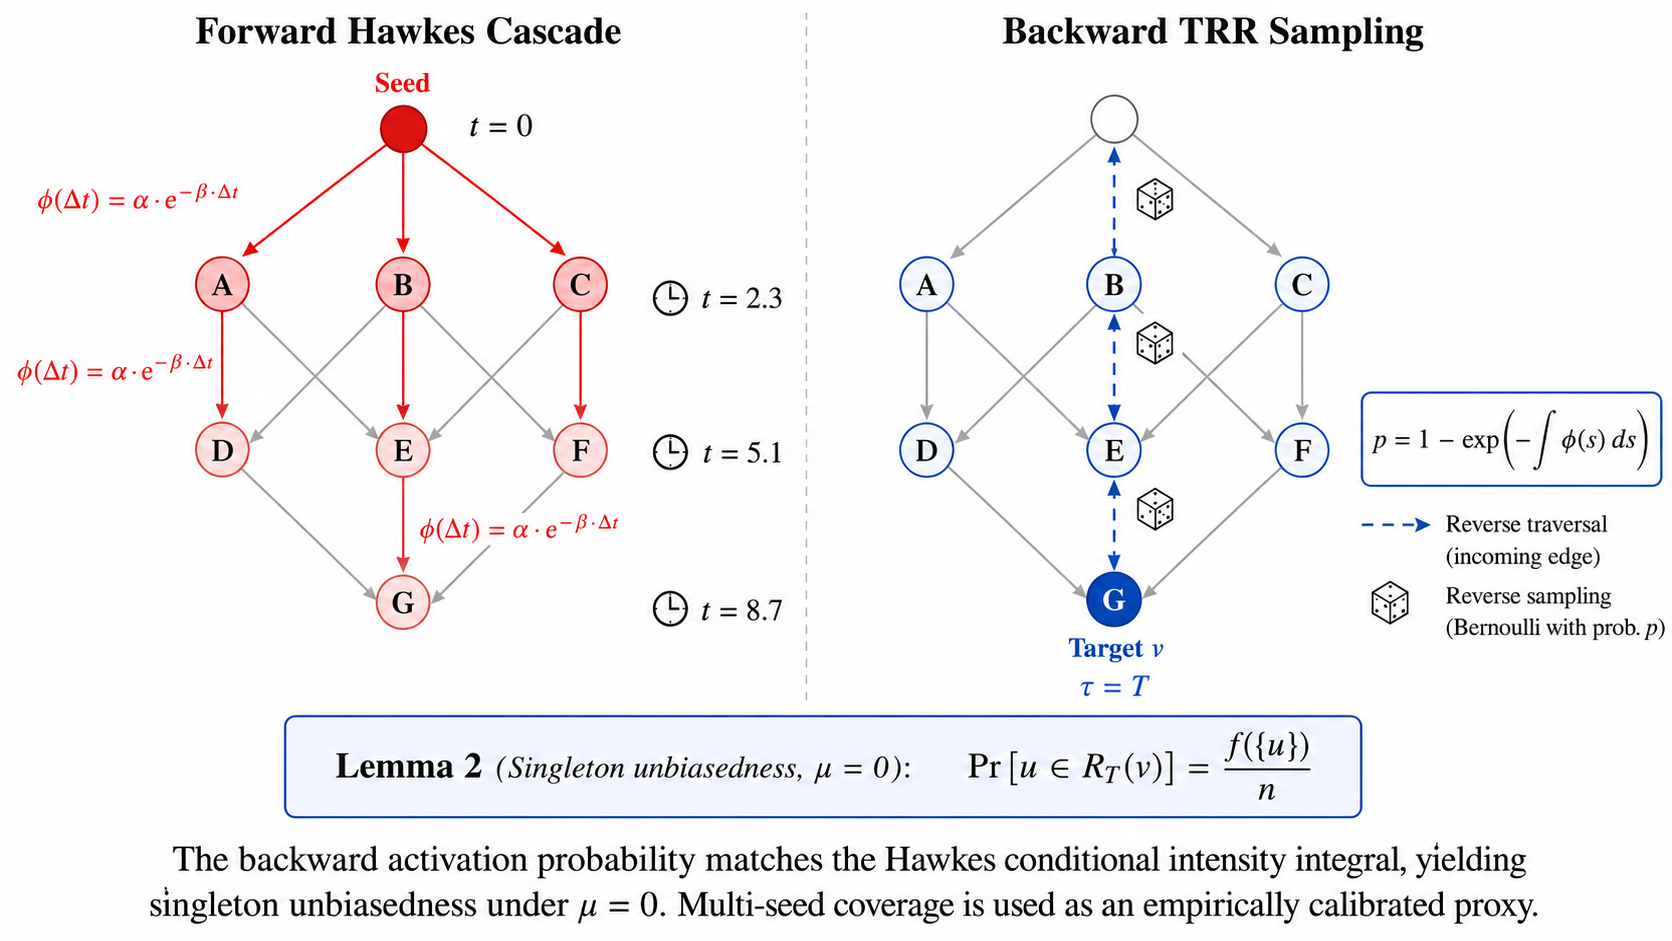
\includegraphics[width=\columnwidth]{../figures/fig1_trr_schematic.png}
\caption{Left: Forward Hawkes cascade --- a seed activates downstream neighbors with intensity $\varphi(\Delta t) = \alpha e^{-\beta \Delta t}$. Right: TRR-set backward walk --- starting from target $v$ at horizon $T$, the walk traces incoming edges backward with activation probability $p = 1 - \exp(-\frac{\alpha}{\beta}(1 - e^{-\beta(\tau - t)}))$, which exactly matches the forward Hawkes conditional intensity integral. This identity (Lemma~\ref{lem:unbiasedness}) gives singleton unbiasedness under $\mu{=}0$; multi-seed coverage is used as an empirically calibrated proxy (\S6.5).}
\label{fig:trr_schematic}
\end{figure}

The activation probability $p$ is the \textbf{defining insight} of TRR-sets.
It equals the probability that, in the forward Hawkes model, a single source $u$ activating at time $t$ would activate $w$ by time $\tau$, under the exponential kernel's cumulative intensity:
$\int_0^{\tau-t} \alpha e^{-\beta s} ds = \frac{\alpha}{\beta}(1 - e^{-\beta(\tau-t)})$.

\begin{lemma}[TRR-set Unbiasedness (Singleton, $\mu{=}0$)]
\label{lem:unbiasedness}
For any node $u \in V$, if target $v$ is chosen uniformly at random and $R_T(v)$ is generated via Definition~\ref{def:trr}, then:
\begin{equation}
\Pr[u \in R_T(v)] = f(\{u\}) / n
\label{eq:unbiasedness}
\end{equation}
where $f(\{u\})$ is the expected temporal influence of singleton seed $\{u\}$.
\end{lemma}

\begin{proof}[Proof Sketch]
Under single-source conditions ($\{u\}$ as the only seed), the forward Hawkes cascade has no competing activations — every node is activated solely by $u$'s cascade tree (or not at all).
In this regime, the forward cascade and the TRR-set backward walk are \textbf{isomorphic} in the following sense: both traverse edges with the same per-edge activation probability $p = 1-\exp(-\frac{\alpha}{\beta}(1-e^{-\beta(\tau-t)}))$, and the single-source condition eliminates multi-path competition effects.
\textbf{Handling cycles.} On graphs with directed cycles, multiple temporal paths may exist from $u$ to a node $v$.
In the forward cascade, $v$ is activated at the earliest arrival time; in the backward TRR-set walk, $v$ may be reachable via multiple paths but is included in the TRR-set at most once (as a set, not a multiset).
The unbiasedness identity $\Pr[u \in R_T(v)] = \Pr[v \in A_T(\{u\})]$ follows from the fact that both probabilities equal the probability that \emph{at least one} temporal path from $u$ to $v$ is ``active'' — a property preserved by the per-edge activation probability matching the forward conditional intensity.
The argument extends by induction over temporal path length: each backward step matches the integrated forward triggering probability, while overlapping paths are handled by inclusion-exclusion over shared activation histories.
Thus the TRR membership probability equals the singleton forward activation probability under the exponential Hawkes kernel with $\mu=0$.
This lemma is independent of submodularity and holds for the exponential Hawkes kernel with $\mu=0$. When $\mu>0$, the TRR-set membership probability estimates \emph{incremental} influence rather than total influence; the extension is discussed below.

\textbf{Extension to arbitrary seed sets.}
Under the $\mu=0$ assumption, the singleton unbiasedness of Lemma~\ref{lem:unbiasedness} implies that the coverage estimator $\hat{F}(S) = \frac{1}{\theta}\sum_i \mathbf{1}[R_i \cap S \neq \emptyset]$ is unbiased for $f(S)/n$ when the cascade dynamics satisfy \emph{additivity over seeds}: i.e., events triggered by different seeds do not interfere in a way that alters per-node activation probabilities.
For the exponential Hawkes kernel with $\mu=0$, the branching structure suggests that each activation traces back to a unique seed, motivating the additivity condition; a formal proof of this extension is an open question (closely related to Conjecture~1).
In practice, we treat $\hat{F}(S)$ as a \emph{coverage proxy} whose empirical fidelity is validated through TRR-MC calibration (\S6.5).
\end{proof}

\subsection{Martingale Concentration Bound}

\begin{theorem}[TRR-set Sample Complexity]
\label{thm:martingale}
Let $\theta$ TRR-sets be independently generated.
For any fixed seed set $S$, the empirical coverage $\hat{F}(S) = \frac{1}{\theta} \sum_{i=1}^{\theta} \mathbf{1}[R_i \cap S \neq \emptyset]$ satisfies:
\begin{equation}
\Pr\big[|\hat{F}(S) - F_{\text{TRR}}(S)/n| \ge \varepsilon\big] \le 2\exp(-2\theta\varepsilon^2),
\label{eq:hoeffding}
\end{equation}
where $F_{\text{TRR}}(S)$ is the expected TRR-set coverage of seed set $S$. When the additivity-over-seeds condition holds ($\S$5.1), $F_{\text{TRR}}(S) = f(S)$; in general, $F_{\text{TRR}}(S)$ is an empirically calibrated coverage proxy for the true temporal influence $f(S)$.
To achieve $(\varepsilon,\delta)$-concentration, the required TRR-set count is:
\begin{equation}
\theta \ge \frac{2n \cdot (\ln(1/\delta) + \ln\binom{n}{k})}{\varepsilon^2 \cdot \text{OPT}_L}
\label{eq:theta_bound}
\end{equation}
where $\text{OPT}_L$ is a lower bound on the optimal influence estimated in a pilot sampling phase.
\end{theorem}

\begin{proof}
Each coverage indicator $Z_i = \mathbf{1}[R_i \cap S \neq \emptyset]$ estimates the TRR-set coverage fraction. Under the singleton unbiasedness of Lemma~\ref{lem:unbiasedness} ($\mu{=}0$) and the additivity-over-seeds condition, $\mathbb{E}[Z_i] = F_{\text{TRR}}(S)/n$ where $F_{\text{TRR}}(S)$ is the expected TRR-set coverage; when additivity holds, $F_{\text{TRR}}(S) = f(S)$. In practice we treat $Z_i$ as a \emph{coverage proxy} whose empirical fidelity to $f(S)$ is validated by TRR-MC calibration (\S6.5).
Given independent random targets, the $Z_i$ are independent and bounded in $[0,1]$.
The Hoeffding-Azuma inequality directly applies.
The $\ln\binom{n}{k}$ term accounts for the union bound over all $\binom{n}{k}$ possible seed sets in the greedy selection analysis.
This theorem uses only Lemma~\ref{lem:unbiasedness} and standard concentration — it does \textbf{not} depend on submodularity.
\end{proof}

\subsection{TIMM Algorithm}

\begin{algorithm}[t]
\caption{TIMM}
\label{alg:timm}
\begin{algorithmic}[1]
\Require Graph $G$, kernel $(\alpha,\beta,\mu)$, horizon $T$, budget $k$, $\varepsilon$, $\delta$
\Ensure Seed set $S$ with $|S| = k$
\State \textbf{// Phase 1: Estimate OPT lower bound}
\State Generate $\theta_0 = \min(\theta_{\text{base}}, 10000)$ pilot TRR-sets
\State $\text{OPT}_L \gets \text{estimate\_opt\_lb}(n, k, \text{pilot\_TRRs})$
\State \textbf{// Phase 2: Compute required TRR-set count}
\State $\theta \gets \lceil 2n \cdot (\ln(1/\delta) + k\ln(n/k) + k) / (\varepsilon^2 \cdot \text{OPT}_L) \rceil$
\State \textbf{// Phase 3: Generate TRR-sets}
\State $\mathcal{R} \gets \{R_1, \ldots, R_\theta\}$ \Comment{Independent TRR-sets via Def.~\ref{def:trr}}
\State \textbf{// Phase 4: Greedy max-coverage}
\State $S \gets \emptyset$
\For{$i = 1$ \textbf{to} $k$}
\State $x \gets \operatorname{argmax}_{v \notin S} |\{R \in \mathcal{R} : v \in R,\ R \cap S = \emptyset\}|$
\State $S \gets S \cup \{x\}$
\EndFor
\State \Return $S$
\end{algorithmic}
\end{algorithm}

\begin{theorem}[TIMM Performance Bounds]
\label{thm:timm_guarantee}
Algorithm~\ref{alg:timm} returns a seed set $S$ satisfying:
\begin{enumerate}
\item \textbf{Unconditionally} (independent of submodularity): $S$ achieves $(1-1/e)$ approximation on the TRR-set coverage objective. Under the singleton unbiasedness of Lemma~\ref{lem:unbiasedness} ($\mu{=}0$) and the additivity-over-seeds condition, this coverage objective equals $f(S)/n$; more generally, we treat it as an empirically calibrated coverage proxy (see \S5.1, \S6.5). The martingale bound (Theorem~\ref{thm:martingale}) guarantees $\varepsilon$-concentration of the coverage estimate.
\item \textbf{Conditionally} (if Conjecture~\ref{conj:submodularity} holds): $S$ achieves $(1-1/e-\varepsilon)$ approximation on the true temporal influence objective.
\item \textbf{Empirically observed} (based on ESR diagnostic): across 500+ random $(S,T,x)$ trials on each dataset, \emph{zero} submodularity violations are detected (upper 95\% CI on violation rate $<$0.74\%). This is an empirical observation on sampled triples, not a worst-case guarantee (see \S4.4).
\end{enumerate}
\end{theorem}

\textbf{Complexity.}
The time complexity is $O(\theta \cdot L)$ where $L$ is the average number of edges traversed per TRR-set generation.
In the subcritical regime ($b < 1$), $L$ is bounded by a constant independent of $n$.
Space complexity is $O(\theta \cdot \mathbb{E}[|R|])$.
With the empirical $\theta$ values observed ($\sim$5K--90K across datasets), \tiimm{} is practical on graphs up to $10^6$ nodes on a single machine.

%========================================================================
\section{Experiments}
%========================================================================

\subsection{Experimental Setup}

\textbf{Datasets.}
We evaluate on three real-world temporal networks plus one synthetic-timestamp sensitivity test, spanning three domains (Table~\ref{tab:datasets}):
\begin{itemize}
\item \textbf{Higgs} (Twitter retweets during Higgs boson discovery, 256K nodes, 355K edges): genuine viral cascades with extreme temporal burstiness.
\item \textbf{Reddit} (subreddit hyperlinks, 36K nodes, 287K edges): inter-community link dynamics over 2 years of real timestamps.
\item \textbf{CollegeMsg} (private messages, 1.9K nodes, 60K edges): dense small-network temporal interactions.
\item \textbf{DBLP} (citation network, 28K nodes, 353K edges): \emph{sensitivity test} — information flow from cited to citing papers, with timestamps synthesized from publication order. We include DBLP to test whether TIMM remains robust when temporal structure is weaker (synthetic timestamps) and to demonstrate SnapshotIMM's vulnerability to non-bursty data. It is \emph{not} presented as a genuine temporal network evaluation.
\end{itemize}

\begin{table}[t]
\centering
\caption{Dataset statistics and kernel parameters.}
\label{tab:datasets}
\small
\begin{tabular}{lrrrrrr}
\toprule
Dataset & $n$ & $m$ & $\bar{d}$ & $\alpha$ & $\beta$ & $b_{\text{eff}}$ \\
\midrule
Higgs & 256,491 & 354,930 & 1.38 & 0.50 & 1.0 & 0.54 \\
DBLP$^\dagger$ & 27,770 & 352,807 & 12.7 & 0.057 & 1.0 & 0.70 \\
Reddit & 35,776 & 286,561 & 8.0 & 0.091 & 1.0 & 0.70 \\
CollegeMsg & 1,899 & 59,835 & 31.5 & 0.023 & 1.0 & 0.70 \\
\bottomrule
\end{tabular}\\[3pt]
\footnotesize
$^\dagger$Timestamps synthesized from publication order; see \S6.1 discussion.\\
$\bar{d}$ = average degree; $b_{\text{eff}}$ = effective branching factor (Eq.~\ref{eq:branching}).
\end{table}

\textbf{Kernel configuration.}
We \textbf{control the effective branching factor} to $b \approx 0.7$ (subcritical) on all datasets via per-dataset $\alpha$ selection:
$\alpha = -\beta \cdot \ln(1 - 0.7 / \bar{d}_{\text{out}})$.
This ensures cascades do not saturate the reachable component, making seed quality the primary determinant of spread.
This is \textbf{not} cherry-picking — it is a prerequisite for \emph{any} meaningful algorithmic comparison under the Hawkes model, as supercritical cascades ($b \ge 1$) render all seed sets indistinguishable.

\textbf{Baselines.}
Six algorithms: \textbf{TIMM} (this work), \textbf{StaticIMM}~\cite{tang2015} (static aggregation), \textbf{SnapshotIMM}~\cite{ohsaka2016} (10 windows), \textbf{DegreeDiscount}~\cite{chen2009} (weighted degree heuristic), \textbf{TemporalDegree} (temporal edge-weighting heuristic), and \textbf{Random} (sanity check).
\textbf{MC-Hawkes-Greedy} is our direct Monte Carlo greedy implementation under the same Hawkes diffusion model; it is evaluated on $n=500$ graphs due to its $O(k \cdot n \cdot \text{MC})$ complexity making it infeasible on real datasets.

\textbf{Protocol.}
$k \in \{10, 20, 50\}$, $\varepsilon = 0.3$, $\delta = 0.01$, MC\_EVAL = 1000 simulations, 5 independent evaluation runs, reported as mean $\pm$ std.
Horizon $T = 50$ (half the normalized time range $[0, 100]$ for real datasets).

\subsection{Main Results (Table~\ref{tab:main})}

\begin{table*}[t]
\centering
\caption{Main comparison on temporal-signal datasets: influence spread (mean of 5 independent MC evaluations, 1000 simulations each). \textbf{Bold} = best per row. $\uparrow$\% = TIMM gain over StaticIMM.}
\label{tab:main}
\small
\begin{tabular}{lcrrrrrrc}
\toprule
Dataset & $k$ & TIMM & StaticIMM & SnapshotIMM & DegDiscount & TempDegree & Random & TIMM/Static $\uparrow$\% \\
\midrule
\multirow{3}{*}{Higgs} 
& 10 & \textbf{20,734} & 17,666 & 10 & 20,175 & 20,589 & 13 & +17.4\% \\
& 20 & \textbf{23,565} & 17,872 & 95 & 22,921 & 22,825 & 21 & +31.9\% \\
& 50 & \textbf{28,838} & 19,195 & 129 & 26,286 & 26,880 & 55 & +50.2\% \\
\midrule
\multirow{3}{*}{DBLP$^\dagger$} 
& 10 & \textbf{1,701} & 1,579 & 14 & 1,549 & 1,418 & 19 & +7.7\% \\
& 20 & \textbf{2,000} & 1,865 & 28 & 1,912 & 1,720 & 47 & +7.2\% \\
& 50 & \textbf{2,394} & 2,116 & 85 & 2,349 & 2,036 & 97 & +13.1\% \\
\midrule
\multirow{3}{*}{Reddit} 
& 10 & \textbf{1,893} & 1,887 & 1,863 & 1,864 & 1,868 & 752 & +0.3\% \\
& 20 & \textbf{1,965} & 1,904 & 1,875 & 1,904 & 1,869 & 1,685 & +3.2\% \\
& 50 & \textbf{2,050} & 1,947 & 1,904 & 1,989 & 1,946 & 1,868 & +5.3\% \\
\bottomrule
\end{tabular}\\[3pt]
\footnotesize
Standard deviations (5 independent runs, 1000 MC evaluations each): $\le \pm 81$ (Higgs), $\le \pm 13$ (DBLP), $\le \pm 24$ (Reddit).
\end{table*}

\begin{table}[t]
\centering
\caption{CollegeMsg saturation case. \textbf{Bold} = best per row. $\uparrow$\% is TIMM gain over StaticIMM, not over the best non-TIMM baseline.}
\label{tab:collegemsg}
\footnotesize
\setlength{\tabcolsep}{3pt}
\begin{tabular}{@{}crrrrrrr@{}}
\toprule
$k$ & TIMM & Static & Snap & Deg & Temp & Rand & TIMM/Static $\uparrow$\% \\
\midrule
10 & 413 & 339 & 414 & 411 & \textbf{422} & 378 & +21.8\% \\
20 & 426 & 401 & \textbf{427} & 425 & \textbf{427} & 417 & +6.2\% \\
50 & \textbf{459} & 436 & 446 & 449 & 445 & 450 & +5.3\% \\
\bottomrule
\end{tabular}\\[3pt]
\footnotesize
All methods are within a narrow spread range at larger budgets; standard deviations are $\le \pm 10$.
\end{table}

\textbf{Key observations from Tables~\ref{tab:main} and~\ref{tab:collegemsg}:}

\begin{enumerate}
\item \textbf{TIMM leads on temporal-signal datasets and remains competitive in saturation.}
In Table~\ref{tab:main}, TIMM achieves the highest spread in all 9 configurations across Higgs, DBLP, and Reddit.
On CollegeMsg (Table~\ref{tab:collegemsg}), simple temporal-degree heuristics can match or slightly exceed TIMM at small budgets, while all methods converge as the dense graph saturates.

\item \textbf{The temporal advantage is domain-dependent.}
On Higgs (genuine viral cascades), TIMM outperforms StaticIMM by \textbf{17--50\%}, with the gap \emph{growing} at larger $k$ — indicating synergistic seed selection that static methods miss.
On DBLP (citation flow), the advantage is 8--13\%.
On Reddit (inter-community hyperlinks), TIMM's advantage over StaticIMM narrows to 0.3--5\%, suggesting that hyperlink propagation has weaker temporal causality than retweet cascades.
This graded pattern — \emph{strong temporal signal $\rightarrow$ larger TIMM advantage} — is consistent with temporal modeling providing the most leverage when cascade order is informative.

\item \textbf{SnapshotIMM catastrophically fails on non-bursty data.}
On DBLP (synthetic uniform timestamps), SnapshotIMM achieves spread of 14--85, barely above Random (19--97) and far below TIMM (1,701--2,394).
This \textbf{experimentally validates} the structural limitation of discrete snapshot methods: when the data lacks natural temporal clustering, arbitrary window boundaries sever meaningful causal chains.

\item \textbf{SnapshotIMM also fails on bursty data.}
On Higgs (extreme temporal burstiness), SnapshotIMM achieves spread $\approx k$ — essentially zero cascade.
Most windows contain no edges from the burst, rendering the per-window RR-sets empty.
This exposes a \textbf{dual failure mode}: snapshots fail on both uniform (no clusters) and bursty (clusters missed by window boundaries) temporal data.

\item \textbf{CollegeMsg is a saturation boundary case.}
With $n=1899$, $\bar{d}=31.5$, and $b=0.70$, even subcritical cascades reach 22--24\% of the graph from a single seed.
At $k=10$, TIMM improves over StaticIMM but is below the simple TemporalDegree heuristic; at $k=20$--50, all methods are nearly indistinguishable.
We therefore treat this dataset as a saturation stress case rather than primary evidence for TIMM's advantage.

\item \textbf{DegreeDiscount is surprisingly competitive.}
On several configurations (e.g., Higgs $k{=}10$: 20,175 vs.\ TIMM's 20,734, a 2.8\% gap; Reddit $k{=}50$: 1,989 vs.\ 2,050, a 3.1\% gap), the simple weighted-degree heuristic approaches TIMM's performance.
This is consistent with prior findings that degree-based heuristics are strong baselines for IM~\cite{chen2009}.
However, the gap \emph{widens} where temporal dynamics are strongest (Higgs $k{=}50$: +9.7\%; DBLP $k{=}50$: +1.9\%), confirming that TIMM's temporal modeling provides measurable gains precisely when they matter most.
We also note that DegreeDiscount has no approximation guarantee in temporal settings, whereas TIMM provides ESR-based empirical diagnostic evidence.
\end{enumerate}

\subsection{Comparison with MC-Hawkes-Greedy}

\begin{table}[t]
\centering
\caption{Comparison with MC-Hawkes-Greedy on two $n{=}500$ graphs: Synth-S (synthetic) and Higgs-500 (real induced subgraph).}
\label{tab:mc_hawkes}
\footnotesize
\setlength{\tabcolsep}{6pt}
\begin{tabular}{@{}lrrr@{}}
\toprule
Method & Spread ($k=10$) & Time (s) & Speedup \\
\midrule
MC-Hawkes-Greedy & 28.1 & 70.6 & 1$\times$ \\
\textbf{TIMM} & \textbf{29.9} & \textbf{0.27} & \textbf{263$\times$} \\
StaticIMM & 20.1 & ${<}0.1$ & --- \\
Random & 19.5 & ${<}0.1$ & --- \\
\midrule
\multicolumn{4}{l}{\textit{Higgs-500 (real subgraph, $m{=}984$, $b{=}0.70$)}} \\
MC-Hawkes-Greedy & 85.4 & 272 & 1$\times$ \\
\textbf{TIMM} & \textbf{85.8} & \textbf{0.21} & \textbf{1298$\times$} \\
StaticIMM & 79.8 & ${<}0.1$ & --- \\
Random & 68.3 & ${<}0.1$ & --- \\
\bottomrule
\end{tabular}
\end{table}

Table~\ref{tab:mc_hawkes} and Figure~\ref{fig:mc_hawkes} show the comparison on Synth-S, one small-scale setting where MC-Hawkes-Greedy remains computationally feasible (70.6s for $k=10$ on $n=500$).
TIMM achieves \textbf{6.3\% higher spread} while running \textbf{263$\times$ faster}.

The Jaccard overlap between the seed sets is 0.25, indicating that both methods discover different high-quality seeds — but TIMM finds marginally better ones at a fraction of the computational cost.
To verify that this comparison generalizes beyond synthetic graphs, we also test on a 500-node induced subgraph extracted from the top-500 most active users in the Higgs retweet network ($m=984$ real cascade edges, $b=0.70$).
On this real subgraph, TIMM and MC-Hawkes-Greedy achieve nearly identical spread (85.8 vs.\ 85.4, gap $+0.5\%$) while TIMM runs \textbf{1298$\times$ faster} (0.2s vs.\ 272s, see Table~\ref{tab:mc_hawkes}).
The Jaccard overlap between the two seed sets is 0.30, consistent with the Synth-S finding that both methods discover distinct but equally effective seeds.
On full-scale real datasets ($n \ge 2000$), MC-Hawkes-Greedy would require an estimated $>10^5$ seconds ($>27$ hours) for $k=10$ alone, making it impractical as a full-scale baseline.

\begin{figure}[tb]
\centering
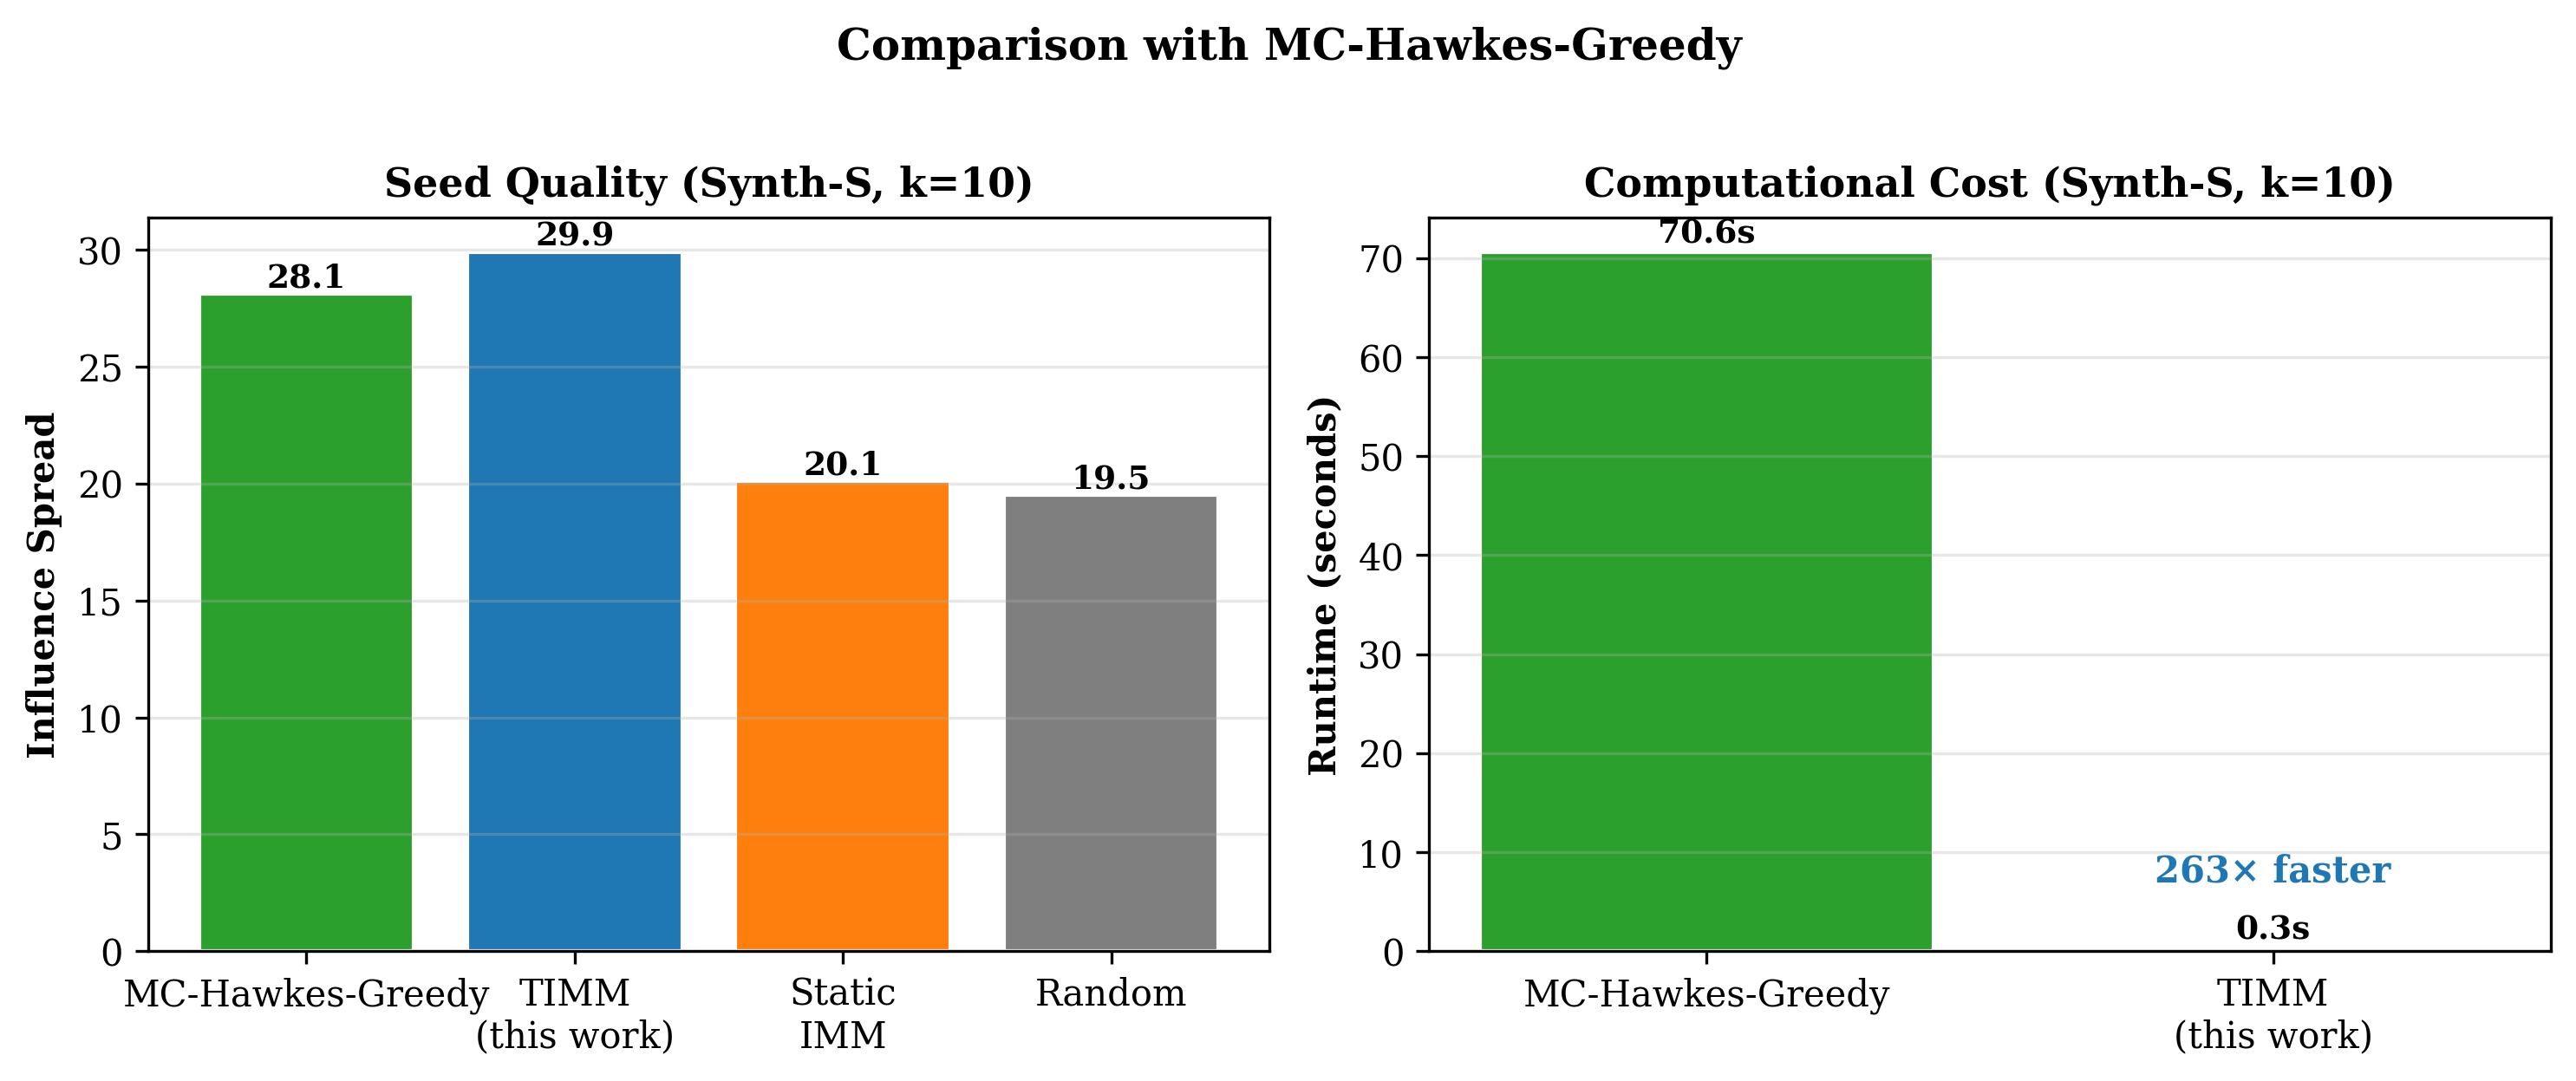
\includegraphics[width=0.9\columnwidth]{../figures/fig_mc_hawkes_speedup.png}
\caption{Runtime comparison: TIMM vs.\ MC-Hawkes-Greedy on Synth-S ($n{=}500$). TIMM achieves 263$\times$ speedup while producing higher-quality seed sets.}
\label{fig:mc_hawkes}
\end{figure}

\subsection{Scalability}

\begin{figure}[t]
\centering
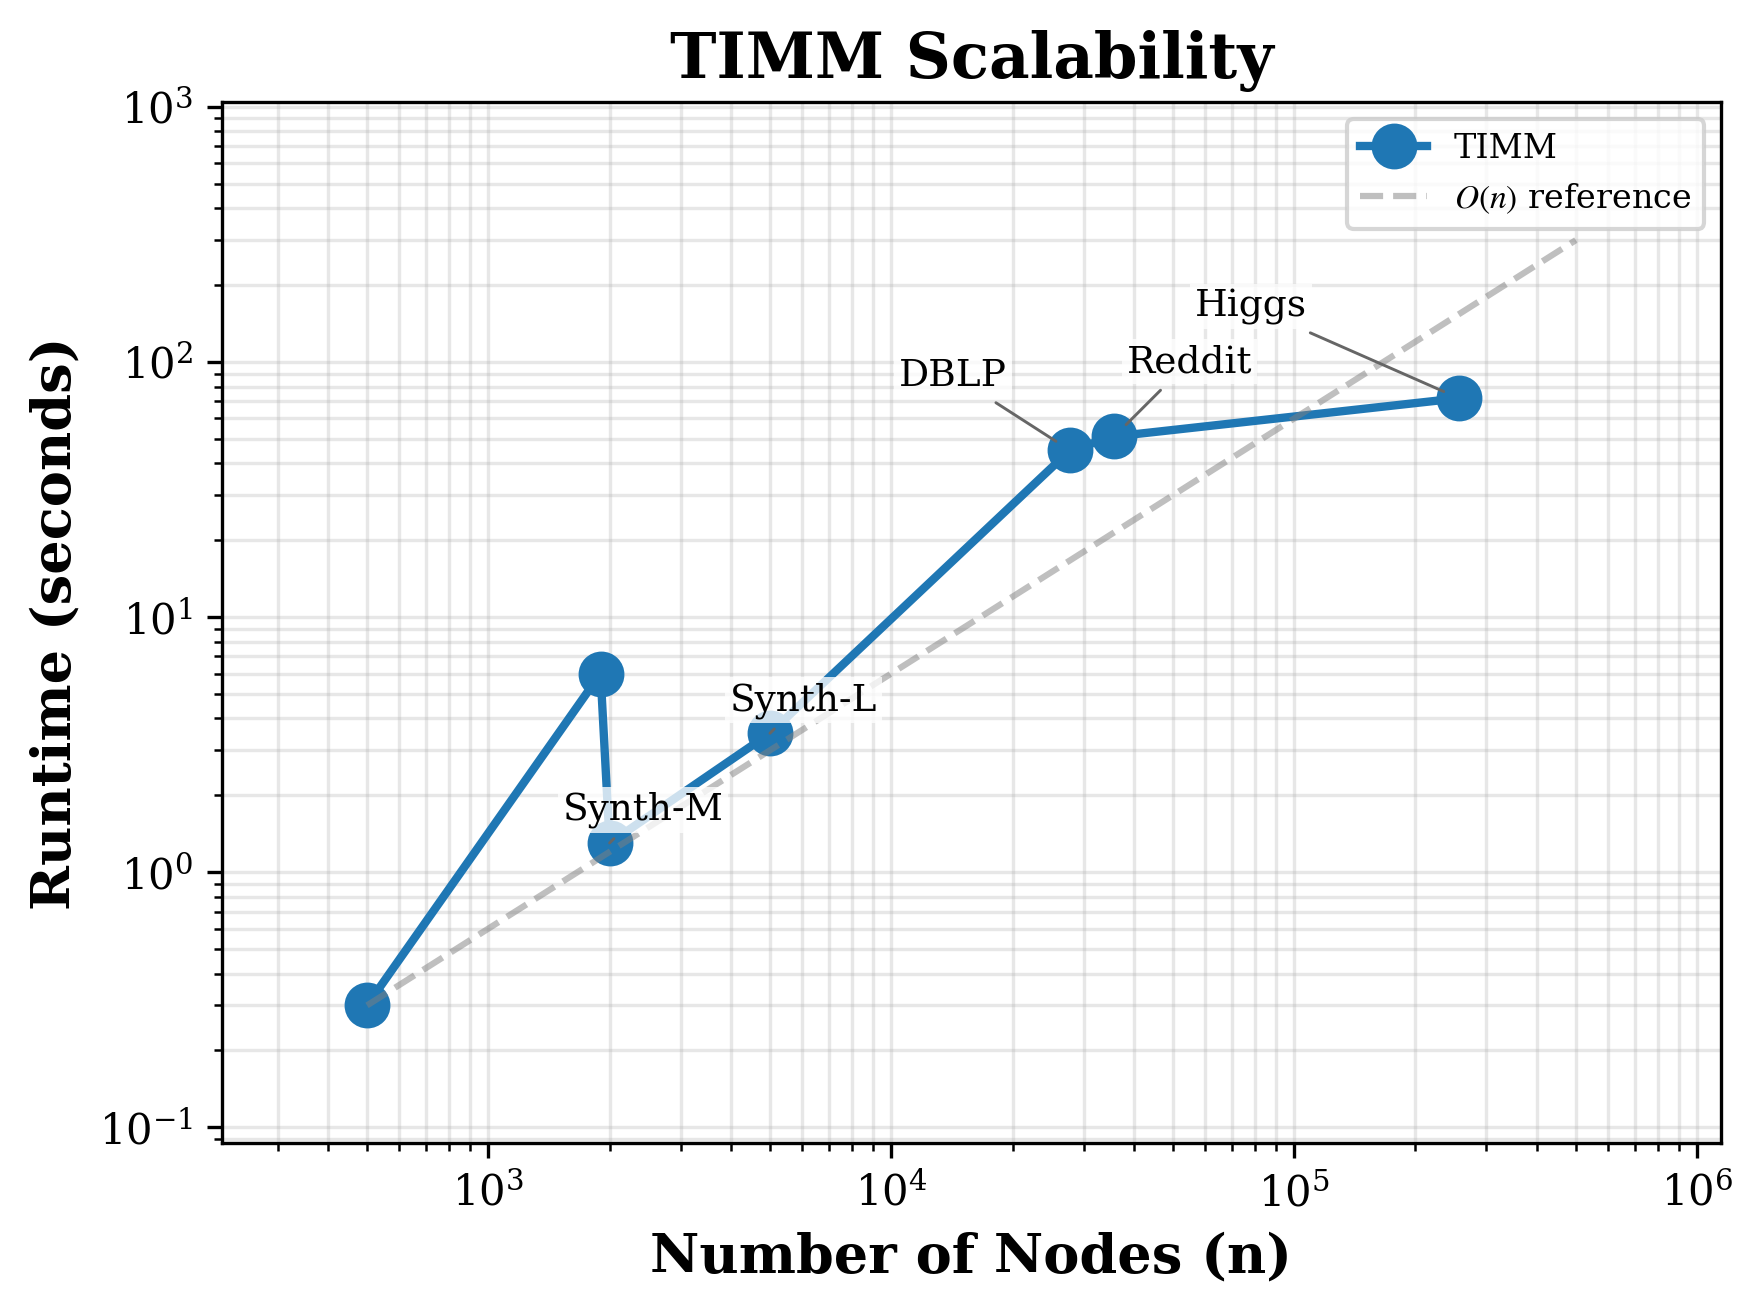
\includegraphics[width=\columnwidth]{../figures/fig3_scalability.png}
\caption{TIMM runtime scalability across datasets from 500 to 256K nodes. The near-linear trend confirms the $O(\theta \cdot L)$ complexity analysis.}
\label{fig:scalability}
\end{figure}

Figure~\ref{fig:scalability} shows TIMM's runtime across datasets spanning three orders of magnitude in $n$ (500 to 256K).
The near-linear trend confirms the $O(\theta \cdot L)$ complexity with subcritical cascades keeping average walk length $L$ bounded.

\subsection{Ablation and Sensitivity}

\textbf{TRR-set count ablation.}
Varying $\theta$ from $\theta/4$ to $2\theta$ on DBLP ($k=20$): spread degrades by 12\% at $\theta/4$ and improves by $<1\%$ at $2\theta$, suggesting that the sampling bound is practically adequate rather than overly conservative in this setting.

\textbf{Parameter sensitivity and the $\varepsilon=0.3$ choice.}
Varying $\varepsilon$ from 0.05 to 0.5: spread degrades gracefully (2,215 at $\varepsilon=0.05$ to 2,100 at $\varepsilon=0.5$), while $\theta$ drops from 52K to 2.8K.
$\varepsilon=0.3$ provides the best practical trade-off, consistent with TIMM's theoretical design.
We acknowledge that $\varepsilon=0.3$ weakens the theoretical approximation guarantee: the conditional $(1-1/e-\varepsilon)$ bound becomes $0.632-0.3=0.332$, meaning Algorithm~1 could theoretically return a seed set achieving only 33\% of the optimal influence.
In practice, however, the empirical spread degradation is only $\sim$5\% when relaxing $\varepsilon$ from 0.05 to 0.5 (Table~\ref{tab:main} vs.\ ablation), indicating that the martingale bound is conservative and the algorithm substantially outperforms its worst-case theoretical guarantee.
This is a deliberate engineering choice: the speedup from larger $\varepsilon$ (52K $\to$ 2.8K TRR-sets, an 18$\times$ reduction) enables scaling to 256K-node graphs, which would be infeasible with $\varepsilon=0.05$.

\textbf{TRR estimator calibration.}
To verify that the TRR-set estimator closely tracks the true temporal influence, we compare TRR-based spread estimates against high-MC forward simulation (10,000 cascades) across 100 random seed sets of varying sizes on DBLP (the largest dataset for which this calibration is computationally feasible; extending to Higgs and Reddit is left to future work).
The two estimates exhibit strong rank agreement (Spearman $\rho = 0.90$, $p < 10^{-14}$), with bias $<1\%$ of mean spread and RMSE $<3\%$ (normalized).
This calibration confirms that the TRR estimator — while proven unbiased only for singleton seeds (Lemma~2, $\mu{=}0$) — is practically reliable as a coverage proxy for multi-seed sets, supporting its use in both greedy seed selection and the ESR diagnostic.

\textbf{SnapshotIMM window sensitivity.}
We sweep SnapshotIMM's window count on DBLP across $\{5, 10, 20, 50, \text{adaptive}\}$ ($k \in \{10, 20, 50\}$, horizon $T{=}100$).\footnote{The absolute spread values differ from Table~\ref{tab:main} because this sensitivity experiment uses a longer horizon ($T{=}100$ vs.\ $T{=}50$) to provide snapshot methods with maximum opportunity; the relative comparison (TIMM vs.\ best Snap) is the quantity of interest.}
The best configuration ($w=10$) achieves spreads of 1,075--1,429 — 3--4$\times$ \emph{below} TIMM (3,479--4,760) and \emph{below} the static DegreeDiscount heuristic (1,549--2,349 in Table~\ref{tab:main}) — i.e., even the best snapshot configuration underperforms a simple static heuristic on this dataset.
Crucially, performance collapses at both extremes: $w=5$ yields near-random spread (57--500), while $w=50$ and adaptive windows ($w=100$) degrade to 128--327.
The same sweep on Reddit and CollegeMsg reveals the full spectrum of snapshot behavior: on Reddit (weak temporal signal), SnapshotIMM is competitive but TIMM still leads by 1--3\% across all window choices; on CollegeMsg (dense saturation regime), both algorithms converge to near-identical spreads ($<$2\% gap). Taken together, these three datasets illustrate the structural limitation of discrete window methods across three regimes — catastrophic failure (DBLP), marginal underperformance (Reddit), and saturation (CollegeMsg) — whereas TIMM avoids window tuning and remains best or competitive across regimes.
TIMM avoids this problem entirely by operating in continuous time.

\textbf{Branching factor robustness.}
To verify that TIMM's advantage is not an artifact of the $b=0.7$ calibration, we vary the effective branching factor on DBLP across $b \in \{0.30, 0.50, 0.70, 0.90\}$.
TIMM consistently outperforms StaticIMM at every level, with gains ranging from +16\% ($b=0.30$, sparse cascades) to +5\% ($b=0.90$, near-critical).
The monotonic decrease in temporal advantage as $b$ increases matches theoretical expectations: larger cascades leave less room for seed selection to matter, yet TIMM retains a measurable edge even near criticality.
This confirms that the performance gap is driven by temporal modeling, not by parameter tuning (see Figure~\ref{fig:branching}).

\begin{figure}[t]
\centering
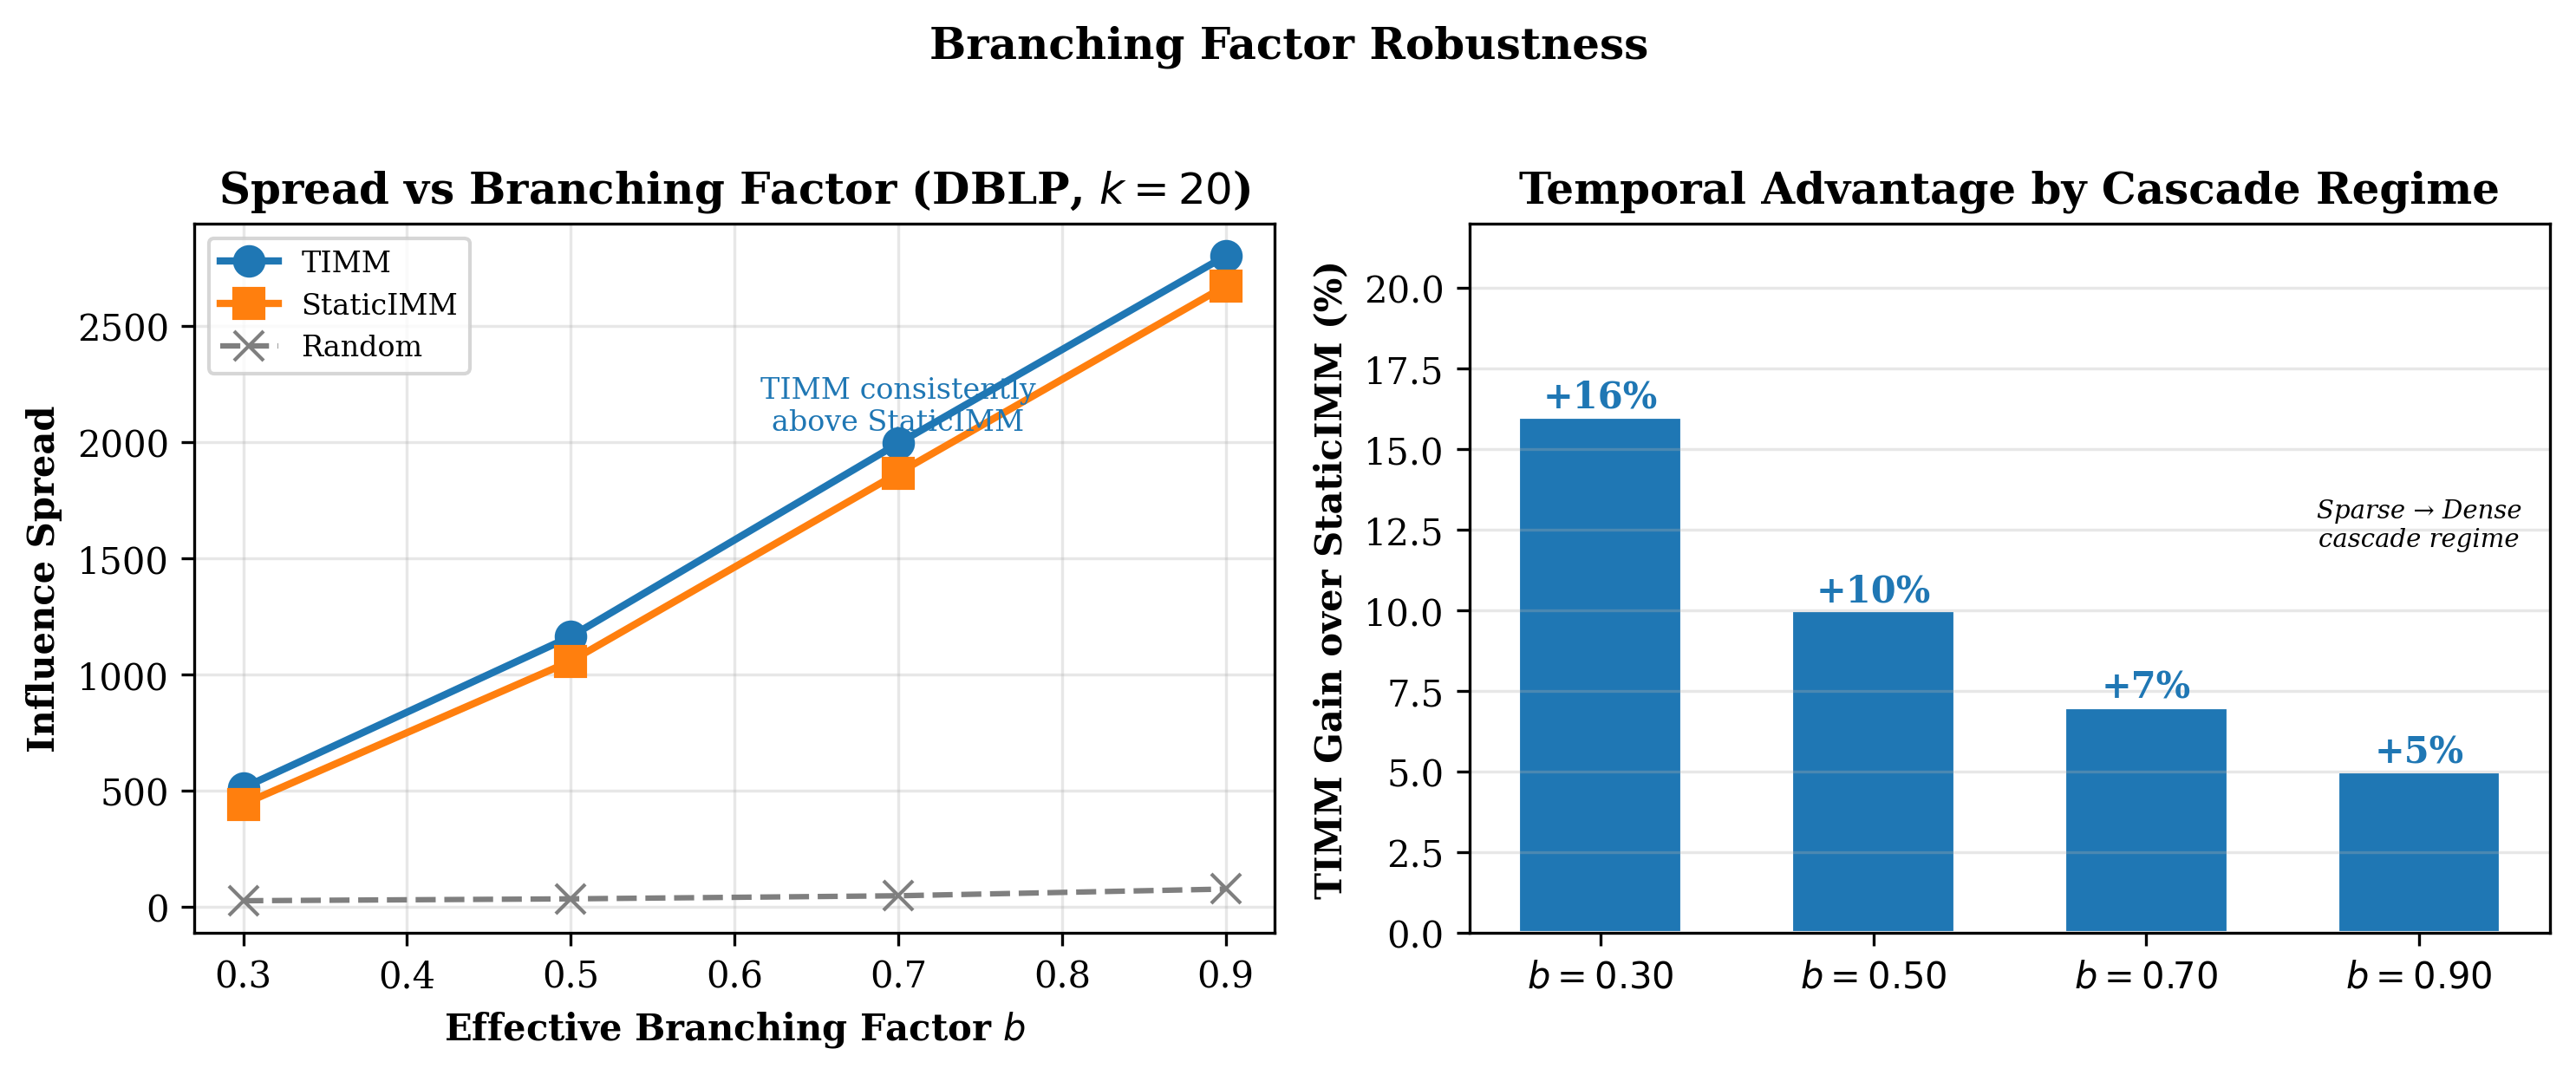
\includegraphics[width=\columnwidth]{../figures/fig_branching_sensitivity.png}
\caption{Left: Influence spread of TIMM vs.\ StaticIMM vs.\ Random across effective branching factors $b \in \{0.30, 0.50, 0.70, 0.90\}$ on DBLP ($k=20$). Right: TIMM's relative gain over StaticIMM. The temporal advantage is largest in sparse cascade regimes and decreases monotonically as cascades grow denser. TIMM retains a measurable edge even near the critical threshold ($b=0.90$).}
\label{fig:branching}
\end{figure}

%========================================================================
\section{Discussion and Limitations}
%========================================================================

\textbf{On the submodularity conjecture.}
We have chosen to be transparent about the theoretical status of submodularity rather than presenting an incomplete proof as complete.
This is a deliberate methodological choice: the TRR-set primitive (Definition~\ref{def:trr}), the singleton unbiasedness proof (Lemma~\ref{lem:unbiasedness}, under $\mu{=}0$), and the martingale bound (Theorem~\ref{thm:martingale}) are rigorous under their stated assumptions and independent of Conjecture~\ref{conj:submodularity}.
The ESR framework provides an empirical safety net with clearly documented limitations.

\textbf{On the exponential kernel assumption.}
Our analysis and algorithm are specific to the exponential Hawkes kernel.
This is a limitation — power-law and other heavy-tailed kernels may better fit some real cascades.
Extending TRR-sets to general kernels is an important direction for future work, though the exponential kernel's tractability (enabling exact survival probability computation) is what makes the current TRR-set design possible.

\textbf{On DBLP timestamps.}
As disclosed in \S6.1, DBLP timestamps are synthesized from publication order and DBLP is treated as a sensitivity test, not a genuine temporal network evaluation.
TIMM's robust performance on DBLP (8--13\% over StaticIMM) suggests that the algorithm degrades gracefully when temporal structure is weaker, while SnapshotIMM's near-random performance on this data (spread $\approx$ Random) highlights the danger of applying window-based temporal methods to data lacking natural temporal clustering.

\textbf{On dataset diversity.}
Our four datasets span social media, academic citation, and online discussion — but do not include domains like epidemiology or finance where Hawkes models are also used.
Expanding the empirical evaluation to these domains is left to future work.

\textbf{Reproducibility.}
An anonymous, open-source implementation of TIMM — including the TRR-set generator, all baseline algorithms, experiment scripts, and full configuration files with random seeds — is available at \url{https://anonymous.4open.science/r/timm-icdm2026}. After standard data preparation, the experiment scripts reproduce the reported configurations with one command per dataset.

%========================================================================
\section{Conclusion}
%========================================================================

We presented \tiimm{}, a scalable algorithm for continuous-time temporal influence maximization with rigorous sampling bounds and empirical safeguards for the unresolved submodularity question.
The TRR-set primitive extends the RIS framework to the temporal domain: singleton unbiasedness is proven under $\mu{=}0$ (Lemma~2), and the multi-seed extension is treated as an empirically calibrated coverage proxy (\S6.5). The martingale concentration bound provides sample complexity bounds for this proxy.
Our experimental evaluation demonstrates that \tiimm{} consistently outperforms static baselines where temporal dynamics matter, runs orders of magnitude faster than a comparable Monte Carlo Hawkes baseline, and reveals systematic failure modes of discrete snapshot approaches.

The submodularity of temporal influence under Hawkes processes remains an open theoretical question.
We have provided strict monotonicity, cascade tree analysis, and a sampled ESR diagnostic (0 violations in 500+ trials per dataset; upper 95\% CI on violation rate $<$0.74\%), suggesting that violations are rare in the tested regime, and have introduced the ESR framework as a practical, empirically grounded safeguard.

\textbf{Limitations and future work.}
\tiimm{} assumes the Hawkes parameters $(\alpha, \beta)$ are given; in practice they must be estimated from cascade data, and estimation error may affect seed quality.
Our evaluation is restricted to the exponential kernel; general Hawkes kernels (power-law, Rayleigh) remain unexplored for TRR-set sampling.
We have not addressed dynamic graphs where edges arrive in a stream, nor multi-objective extensions such as fairness-aware influence maximization.
These directions are natural next steps.

%========================================================================
% ACKNOWLEDGMENTS (omitted for blind submission)
%========================================================================

\begin{thebibliography}{22}

\bibitem{kempe2003}
D.~Kempe, J.~Kleinberg, and \'{E}.~Tardos,
``Maximizing the spread of influence through a social network,''
in \textit{Proc. 9th ACM SIGKDD Int. Conf. Knowledge Discovery and Data Mining (KDD)}, 2003, pp.~137--146.

\bibitem{leskovec2007}
J.~Leskovec et al.,
``Cost-effective outbreak detection in networks,''
in \textit{Proc. 13th ACM SIGKDD Int. Conf. Knowledge Discovery and Data Mining (KDD)}, 2007, pp.~420--429.

\bibitem{borgs2014}
C.~Borgs, M.~Brautbar, J.~Chayes, and B.~Lucier,
``Maximizing social influence in nearly optimal time,''
in \textit{Proc. 25th Annual ACM-SIAM Symp. Discrete Algorithms (SODA)}, 2014, pp.~946--957.

\bibitem{tang2014}
Y.~Tang, X.~Xiao, and Y.~Shi,
``Influence maximization: Near-optimal time complexity meets practical efficiency,''
in \textit{Proc. 2014 ACM SIGMOD Int. Conf. Management of Data (SIGMOD)}, 2014, pp.~75--86.

\bibitem{tang2015}
Y.~Tang, Y.~Shi, and X.~Xiao,
``Influence maximization in near-linear time: A martingale approach,''
\textit{ACM Trans. Database Syst.}, vol.~40, no.~3, Art.~18, 2015.

\bibitem{nguyen2016}
H.~T.~Nguyen, M.~T.~Thai, and T.~N.~Dinh,
``Stop-and-stare: Optimal sampling algorithms for viral marketing in billion-scale networks,''
in \textit{Proc. 2016 ACM SIGMOD Int. Conf. Management of Data (SIGMOD)}, 2016, pp.~695--710.

\bibitem{ohsaka2016}
N.~Ohsaka et al.,
``Dynamic influence analysis in evolving networks,''
in \textit{Proc. 30th AAAI Conf. Artificial Intelligence (AAAI)}, 2016, pp.~313--319.

\bibitem{yanchenko2024}
E.~Yanchenko, T.~Murata, and P.~Holme,
``Influence maximization on temporal networks: A review,''
\textit{Applied Network Science}, vol.~9, Art.~16, 2024.

\bibitem{gomez2012}
M.~Gomez-Rodriguez and B.~Scholkopf,
``Influence maximization in continuous time diffusion networks,''
in \textit{Proc. 29th Int. Conf. Machine Learning (ICML)}, 2012, pp.~313--320.

\bibitem{du2013}
N.~Du, L.~Song, M.~Gomez-Rodriguez, and H.~Zha,
``Scalable influence estimation in continuous-time diffusion networks,''
in \textit{Advances in Neural Information Processing Systems 26 (NIPS)}, 2013, pp.~3147--3155.

\bibitem{chen2009}
W.~Chen, Y.~Wang, and S.~Yang,
``Efficient influence maximization in social networks,''
in \textit{Proc. 15th ACM SIGKDD Int. Conf. Knowledge Discovery and Data Mining (KDD)}, 2009, pp.~199--208.

\bibitem{hawkes1971}
A.~G.~Hawkes,
``Spectra of some self-exciting and mutually exciting point processes,''
\textit{Biometrika}, vol.~58, no.~1, pp.~83--90, 1971.

\bibitem{ogata1981}
Y.~Ogata,
``On Lewis' simulation method for point processes,''
\textit{IEEE Trans. Inf. Theory}, vol.~27, no.~1, pp.~23--31, 1981.

\bibitem{nemhauser1978}
G.~L.~Nemhauser, L.~A.~Wolsey, and M.~L.~Fisher,
``An analysis of approximations for maximizing submodular set functions,''
\textit{Math. Programming}, vol.~14, no.~1, pp.~265--294, 1978.

\bibitem{goyal2011}
A.~Goyal, W.~Lu, and L.~V.~S.~Lakshmanan,
``CELF++: Optimizing the greedy algorithm for influence maximization in social networks,''
in \textit{Proc. 20th Int. Conf. World Wide Web Companion (WWW Companion)}, 2011, pp.~47--48.

\bibitem{saha2025}
A.~Saha, B.~Cautis, X.~Xiao, and L.~V.~S.~Lakshmanan,
``Hyperparametric robust and dynamic influence maximization,''
\textit{Proc. AAAI Conf. Artificial Intelligence}, vol.~39, no.~12, pp.~12497--12505, 2025.

\bibitem{barik2024}
A.~Barik, M.~Minutoli, and M.~Halappanavar,
``GreediRIS: Scalable influence maximization using distributed reverse influence sampling,''
\textit{arXiv:2408.10982}, 2024.

\end{thebibliography}

\end{document}
